\documentclass[titlepage]{article}
\usepackage[document]{ragged2e}
\usepackage{amsmath}
\usepackage{graphicx}
\usepackage{indentfirst}
\usepackage{ragged2e}
\usepackage{tikz}
\usepackage{listings}
\usepackage{cite}
\usepackage{pdfpages}
\usepackage[font=it]{caption}
\usepackage{algorithm2e}

%\usepackage[a4paper, margin=1.5in]{geometry}

\RaggedRightParindent = 24pt
\linespread{1.3}


%set code style
\lstdefinestyle{default}
{
	language=C++,
	frame=single,
	tabsize=2,
	numbers=left,
	basicstyle=\small,
	showstringspaces=false,
	captionpos = b
}
%Set Algorithm style
\RestyleAlgo{boxed}
\LinesNumbered
\lstset{style=default}
%opening

\title{Modelling of Nanosecond time-scale Transient response of GaN LEDs \\ \textbf{Project Outline}}
\author{Zachary Humphreys}
\date{\centering ID: 200951438
	\\02/02/2018 \bigskip
\hrule \bigskip
A Thesis Submitted in partial fulfilment of the requirements for the degree of:\\
\textbf{Master of Physics} \\
Under the supervision of Dr. Joachim Rose \\
At the \\
\textbf{Department of Physics}
\bigskip

\includegraphics[scale=0.6]{LiverpoolLogo}
}


\begin{document}

\maketitle

\tableofcontents
\lstlistoflistings
\listoffigures
\listoftables
\listofalgorithms
\newpage

\section*{Declaration}
%\addcontentsline{toc}{Chapter}{Declaration}

I, Zachary Humphreys, hereby declare that this thesis is my own work and effort and that it has not been submitted anywhere for any award. Where other sources of information have been used, they have been acknowledged.
\bigskip \\
\hrule
\textit{Note: As this is the project outline, certain missing information, citations, and other incomplete sections will be labelled in \textbf{bold} font to bring attention to it.}
\hrule

\section{Abstract}
\begin{center}
In this thesis, the light emission properties of Gallium Nitride blue LEDs modelled and explained, particularly of note being the unusual characteristics of one being switched on and off on nanosecond timescales. \\ Switching under these conditions require high voltages in both the forwards and reverse biases and effects that can normally be ignored appear to have much larger effects under these conditions and time scales. \\ Switching LEDs under these time-scales could be of particular use in the calibration of large photo-detectors which focus on detection of very small \textbf{approx\#ofphotons} bursts of photons (such as Neutrino detection experiments)\textbf{findcitationforsuperK}, and so require similarly small, but consistent amounts for calibration.
\end{center}



\section{History \& Introduction}
The very first semiconductor device was the photometer, developed by Von Siemens in 1875 \cite{G3Nsemicomp}(p6) (effectively a primitive solar cell) and hence, from the very inception of semiconductor devices, interaction with light has been closely related. However, it wasn't until 1907 until the electro-luminescence effect was discovered\cite{Sze}[p601] in the form of a point contact with a SiC substrate\cite{Sze}(p608) that emission of light, instead of absorption, was demonstrated. This electro-luminescence was different from radiative emission in both frequency and broadness of spectrum. But it wasn't for yet another 42 years, with the advent of the p-n junction in 1949, that the Light Emitting Diode (LED) as we know it today, was invented.\cite{Sze}(p608)\cite{G3Nsemicomp}(p1). \\
Unfortunately, due to them being made of Indirect Band-gap semiconductors, they had very poor efficiency, and it's progress remained stagnant with a lack of commercialisation\cite{G3Nsemicomp} until the discovery of direct band-gap designs of GaAs in 1962 which had a much higher Quantum Efficiency leading to the first semiconductor laser. Soon after, in 1964, indirect bandgap materials also improved with the process of "doping" (addition of impurities) being discovered.\cite{Sze}(p608) \\
Up until this point, all the discovered LED technology had led to LEDs with spectra in the Infrared to the lower frequency end of the visible spectrum and in 1971, Pankove et. al. reported the first GaN LED and hence, the first LEDs with frequencies in the blue to UV range. \cite{NSD}(p3) However, traditional methods growing crystals of this nature were difficult and would lead to progress in a different technique: Epitaxial growth, where a film of crystal is grown from the surface of another.\cite{G3Nsemicomp}(p8)\cite{Nakamura}(p4). The only problem was, all of the known materials that would produce blue light had short-comings. Of note, was the epitaxial growth of GaN had a lattice mismatch to its best substrate (Sapphire) of 13.8\% , compared with ZnSe (an alternative) on GaAs with a 0.3\% mismatch and could thus easily be grown with few defects, leading to high quality crystals.\cite{G3Nsemicomp}(p11,13)\cite{Nakamura}(p4). \\
These films were generally deposited by either Molecular beam, or metalorganic vapour phase Epotaxy (MOVPE) but would require temperatures of $\approx1300$K and high pressures. As a result of the high rate of defects in GaN at the time ($10^9cm^{-2}$) made ZnSe generally the more popular choice for scientists ($10^3cm^{-2}$) which in turn, led to little research in the area.\cite{Nakamura}\\
In 1990, Nakamura developed a technique (low carrier gas flow MOCVD) for producing high quality, uniform GaN using ammonia, but there was still the challenge of successfully doping it, meaning overcoming Mg acceptor dopant producing complexes with the H \cite{Nakamura}(p5) and finding a suitable Donor n-type. The first GaN pn junction was created in 1991 with an output power of $42\mu W$ and a External Quantum Efficiency of 0.18\% at a wavelength of 430nm (far lower than the minimum 1mW for usefulness.) \\
Only after the discovery of InGaN, and its ideal properties as an active layer in a Double Heterostructure (DH), where it's bandgap was able to be tightly controlled through level of doping with tight control was the first Blue DH LED created, in 1993 which\cite{Nakamura}(p7), in turn, would lead to the first white LED with the addition of a white-phosphor\cite{Sze}(p608), \\The highest External Quantum efficiencies for LEDs are being achieved by GaInP encased in epoxy with 55\%,\cite{EQE} a massive improvement from the earliest versions of LEDs. In comparison, an oil lamp produces approximately $0.1lmW^{-1}$, an incandesceent bulb produces  $16lmW^{-1}$, fluorescent  $70lmW^{-1}$, but an LED will produce  $300lmW^{-1}$\cite{Nakamura}(p3) and the very first pn junction laser diode in visible spectrum of  $\approx 0.1lmW^{-1}$ created by Holonyak in 1962. \cite{Kittel}(p580)\\
Due to their high efficiency and ability to be tightly controlled, LEDs have been implemented in many technologies from simple indicator lights, to room illumination, but recently, they've been considered for calibration of Large photo-detection experiments such as Hyper-K and ANTARES neutrino detection experiments, where they aim to detect the Cherenkov radiation from Muon's produced by neutrinos interacting with matter. These interaction create very short pulses of very few photons of approximately blue colour, and thus, a similar pulse of light would be preferable to calibrate such an experiment.\textbf{CITATIONS NEEDED} \\
For this, the use of Blue, GaN-based LEDs pulsed at nano-second time-scales has been proposed. However, as the lifetime of charge carriers in these materials is on the order of nanoseconds for InGaN/AlGaN DH LEDs\cite{Brailovsky}, it has generally been considered practically impossible to produce such results, and conventional methods for driving LEDs result in rather low switching frequencies on the order of 1GHz. \\ To the contrary, it has been demonstrated that such pulses can be achieved experimentally \textbf{Rose citation?} and thus, an investigation into the mechanism will be conducted as the objective of this thesis, and whether experimental results can be simulated with current models and understanding.


\section{Background Physics and Past Work}
Explain first pn Junction, then pn junction structures, band gaps, LED homo vs hetero structure, and then the fundamental basis of recombination and how it leads to photon emission $\rightarrow$ LEDs. \footnote{(Note to self, Kittel has some good diagrams and basic explainations)}\\
Discuss the Numerical Boltzmann Transport theory based on scattering, and explain that due to time, understanding, and knowledge constraints, this was not a practical option, but still talk about the overview of how it worked.
Discuss drift diffusion equation and how its the basis of much of many of the other theories.
Briefly outline the quantum model, and again discuss how it wasn't practical to go this route with the number of unknowns in the project.
\subsection{Windisch}
In this section will outline the \textbf{Windisch} paper, and it's modelling of instantaneous switching, no loss of charges out of device (LED acts as a charge "Bucket" with $R_{in} = \frac{J}{q\omega} $). Discuss how it assumes negligible Non-radiative recombination.
\subsection{Brailovsky \& Mitin}
Discuss the analytical solution they provide, the massive reverse current predicted, and their neglection of drift current in their analytical model, but how this massive reverse current might actually be the source of the fast-switching of the LED, faster than expected.
\section{Method}
In order to explore the behaviour of the light emitting diode at short time-scales, two simulations were created to explore how different interpretations of the device would affect the results: A "macroscopic" simulation treating the device as a singular object, and a second "microscopic" simulation that took into account of internals of the device. The theoretical foundation for carrier transport in both device simulations was the "Drift-Diffusion" model due to its common usage, and simpler implementation than competing models, such as the Semi-classical Boltzmann Transport Equations that has its basis in the scattering of classical point-like holes and electrons from one set of phase-space coordinates to another.\cite{NSD}[p70-6] \\
The goal of both simulations was to produce plots of the full width half maximum ($\sigma_{FWHM}$) as a function of the number of photons in the pulse, to compare with the real device output.\\
Experimentally, voltage across the diode was ramped up and down over the period of several nanoseconds, with the forwards bias injecting charges, and the reverse bias pulling any remaining charges that hadn't combined, out of the device. In both models, to match the experimental conditions, the applied voltage to the diode was modelled as a tent map with the equations:
\begin{eqnarray}
	V(t) = \begin{cases}
	\alpha t &t < t_{trans}\\
	\alpha(2t_{trans} - t) &t \geq t_{trans}\\
	\end{cases}
\end{eqnarray}
where $V$ is the bias voltage, $t$ is the time, $t_{trans}$ is the transition time from voltage ramp up to voltage ramp down, and $\alpha$ is the voltage ramp scale (found experimentally to be $4Vns^{-1}$). This is an approximation to the experiment as it is not possible to switch instantly from forwards to backwards, with a more realistic model expecting some rounding to the graph graph during switching on, and switching from forwards to backwards. 
\begin{figure}[t]
	\hrule
	\centering
	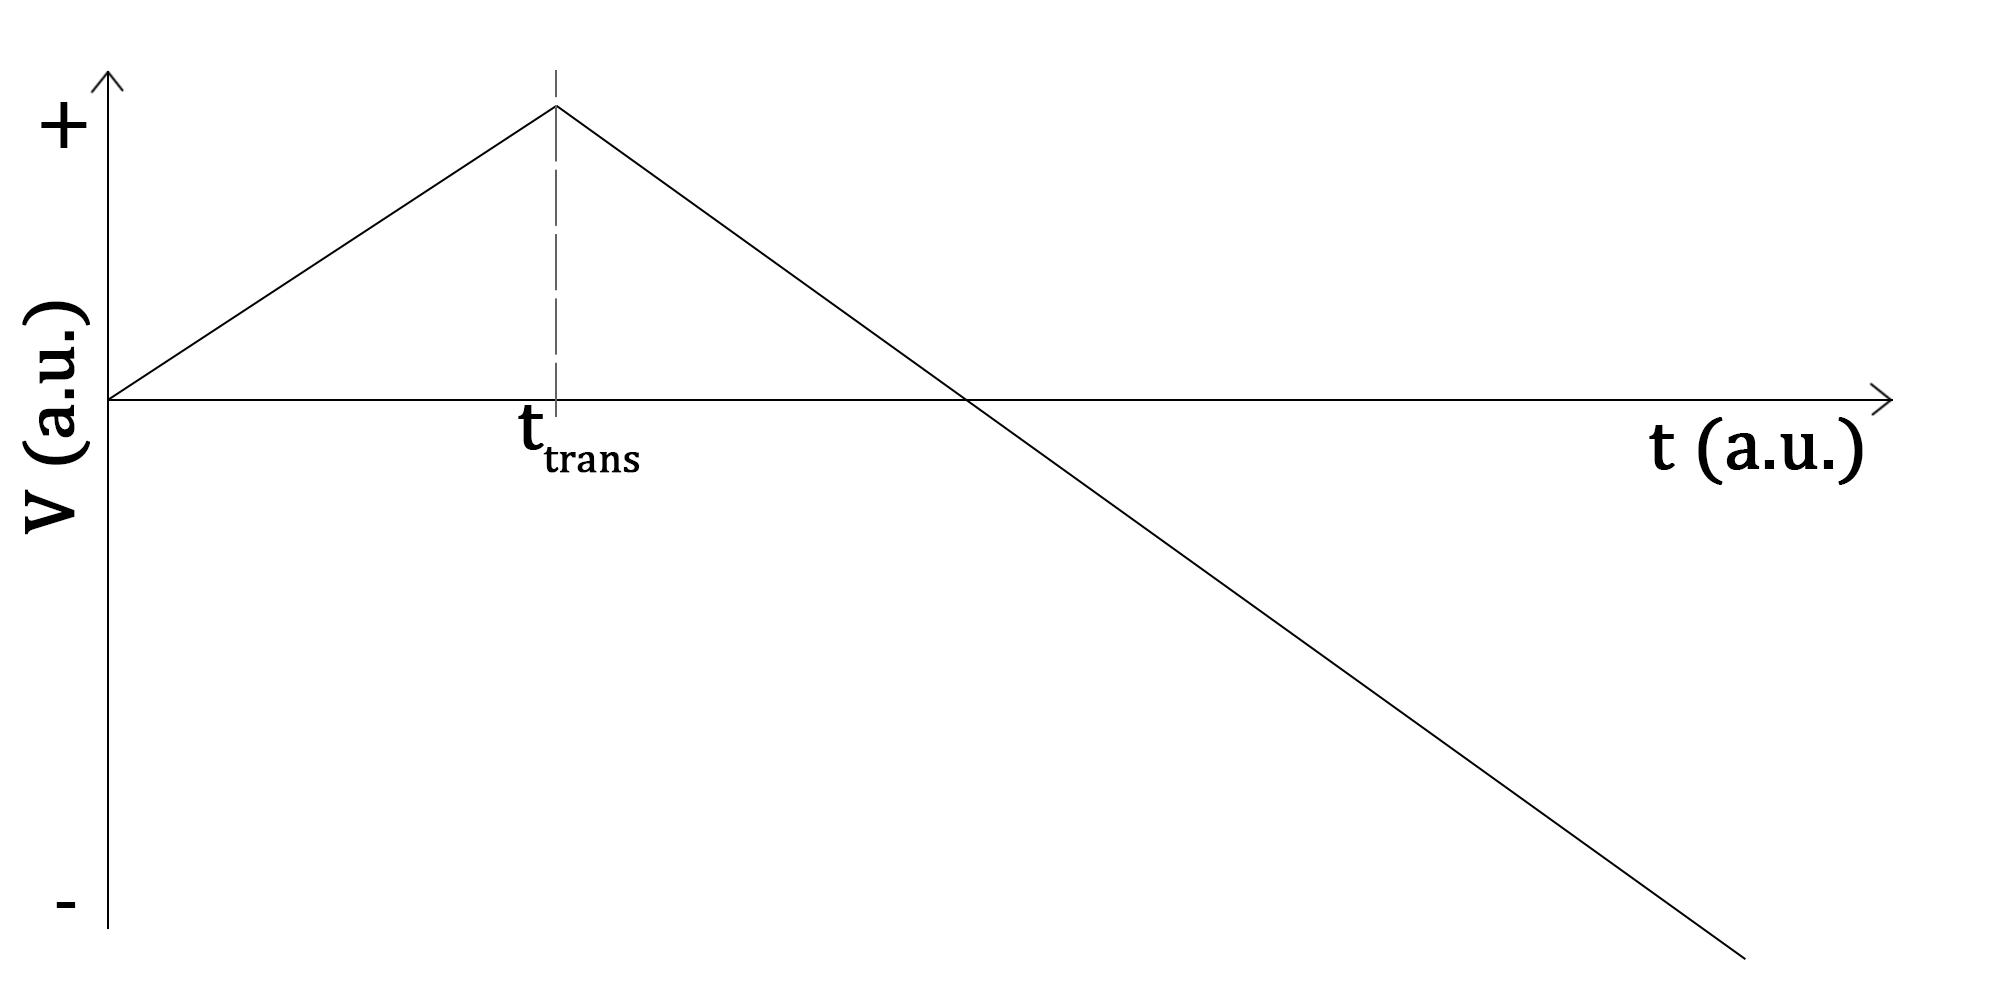
\includegraphics[scale=0.12]{Figures/V_tent}
	\caption{\label{graph:V_tent}Graph of the approximate shape of the voltage ramp up and down used experimentally.}
	\hrule
\end{figure}
\subsection{"Macroscopic" Model}
\subsubsection{Conceptual Overview}
\begin{figure}[t]
	\hrule
	\centering
	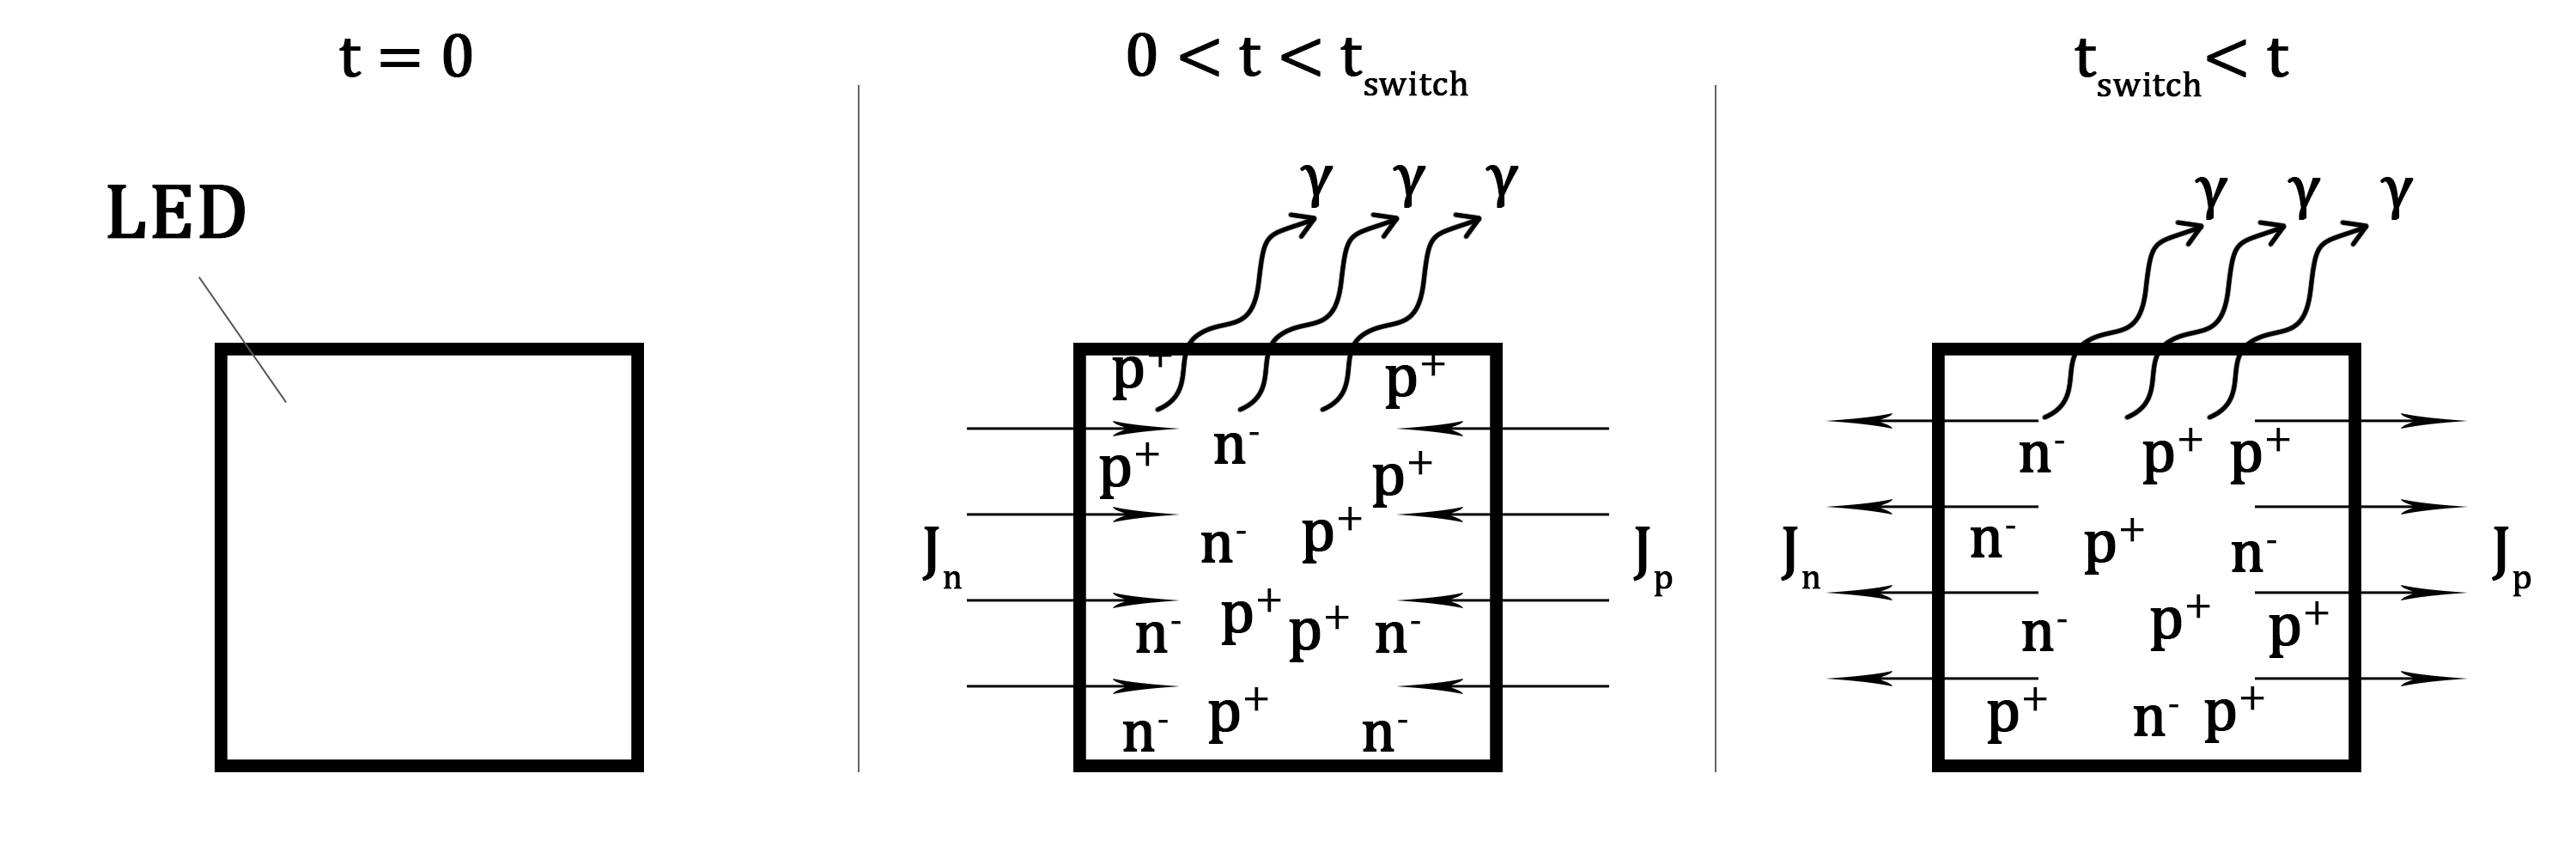
\includegraphics[scale=0.12]{Figures/Bucket_overview}
	\caption{\label{fig:bucketOverview}This figure displays the concept behind the macroscopic model where after time, $t=0$, electrons and holes ($n^-$ and $p^+$ respectively) are injected by currents $J_n$ and $J_p$ until the switch time, where upon the currents are reversed until all the charges have either combined to create photons ($\gamma$), or have been removed.}
	\hrule
\end{figure}
In this simulation, the device was modelled as a single, complete object where charges would be injected, and photons ejected as a result of holes and electrons in the device combining (fig.\ref{fig:bucketOverview}). This interpretation would be similar to treating the device to that of a leaky capacitor under Direct Current operation. This is a not-entirely unrealistic as "real" LEDs do have some small level of capacitance in the form of charge storage and  depletion layer capacitance.\textbf{[CITE: VALEDAR,p30]} This model also means that opposite charges can interact immediately once inside, as the device is treated as so small that the charges are injected in the same place.\\
\subsubsection{Calculating number of charges}
The core calculation for number of charges in the device was done in a discrete time-step manner thus:
\begin{eqnarray}
&n(t) &= n(t-1) + \dfrac{dn}{dt}\Big|_{n=n(t)} \\
\hookrightarrow &n(t) &= n(t-1) + n_J(t) - n_R(t) 
\end{eqnarray}
where $n(t)$ is the number of charges at time t, $n_J(t)$ is number of charges injected at time t, and $n_R(t)$ is the number of charges recombined at time t, with the boundary conditions, $n(0), n(t_{end}) = 0$ with the approximation that Thermal Generation and Recombination were negligible.\\
As both negative and positive charges would be injected at the same rate in this model, it is convenient to work in just one of them (in this case, negative) to simplify certain calculations.\\
To calculate the number of injected charges, the approximation was taken that the LED itself was an Ohmic device, with resistance of $5\Omega$, and using Ohms law:
\begin{eqnarray}
	&I =& \dfrac{V}{R} =  \dfrac{q n_J}{t}\\
\hookrightarrow	&n_J =& \dfrac{V}{qR}t
\end{eqnarray}
where $V$ is the external applied Voltage, $R$ is the resistance, $q$ is the charge on the electron, and $t$ is the amount of time the current is being applied for.\\
The number of charges lost to Radiative Recombination can be found from the  Radiative recombination rate equation given by:\cite{NSD}[p289,306]\cite{Sze}[p614]
\begin{eqnarray}
&R_{rad} =& Bnp\\
\hookrightarrow &R_{rad} =& Bn^2\Big|_{p=n} = n_R 
\end{eqnarray}
where $B$ is the bulk recombination rate constant.\\
\subsubsection{Simulation Algorithms}
The method for finding the number of photons, and FWHM of the associated pulse, was done by running the device simulation over a range of transition times, incrementing the transition time by a small step each loop:\\
\begin{algorithm}[H]
	Create arrays to store FWHM and Number of photons\; 
	\For{$t_{trans} = 0$ to $t_{trans-max}$}
	{
		Carry out the simulation at $t_{trans}$\;
		Save the resulting FWHM and Number of photons to arrays\;
	}
	Print the arrays to file\;
	\caption{Macroscopic outer loop \label{alg:Mac:outer}}
\end{algorithm}
\bigskip
In the program, the size of the transition step, the maximum transition step, and the simulation step can all be determined at run-time via console input at the start.\\
The algorithm for the nested simulation step of the outer loop is defined by Algorithm \ref{alg:Mac:inner}.\\
\begin{algorithm}[H]
	Create array for number of photons and current time\;
	Create Cumulative Radiation variable and set to 0\;
	\While{$n \geq 0$}
	{
		Increment simulation at $t$ by $t_step$\;
		Add time onto end of the time array\;
		Find V at $t$ from tent map\;
		Find $n_J$ from V \;
		Add $n_J$ to $n$\;
		Find $n_R$ (and hence number of photons)\;
		Take $n_R$ from $n$\;
		Add $n_R$ onto end of photon array\;
		Add $n_R$ to cumulative photons.\;
	}
	Use arrays to find FWHM\;
	Send total photons and FWHM to outer loop.\;
	\caption{Macroscopic Inner simulation loop \label{alg:Mac:inner}}
\end{algorithm}
\bigskip
From both of these algorithms, it's clear that the smaller the time step for both the transition time and inner simulation time, the higher the resolution of the data, so generally, the step for the simulation was on the order of $10^{-3}$ times the transition time.\\
To find the FWHM of the pulse, Algorithm \ref{alg:Mac:FWHM} was used. From this method, the error on the FWHM is no more than the width of two bins.\\
\begin{algorithm}[H]
	Find peak photon count bin in the photon array\;
	Find first bin to fall below half this value before and after peak bin\;
	Use bin numbers to find associated times in the time array\;
	Subtract the time from the after-peak bin from the before-peak bin\;
\caption{Finding photon Pulse Full Width Half Maximum \label{alg:Mac:FWHM}}
\end{algorithm}
\bigskip
The resulting data generated by this simulation was then outputted to a .csv file where it could be analysed.

\subsection{"Microscopic" Model}
\subsubsection{Conceptual Overview}
This model was produced to compare the results with the Macroscopic interpretation of the device. It centred around numerically solving the charge Continuity Equations through calculating both the Drift-Diffusion and Poisson's equations:\cite{Frensley}[p21]
\begin{eqnarray}
	&J_n = -q\mu_n n\nabla V + \mu_n n \nabla E_c + q D_n \nabla n\\
	&J_p = -q\mu_p p\nabla V + \mu_p p \nabla E_v - q D_p \nabla p\\
	&\nabla\cdot\vec{D} = \rho
\end{eqnarray}
where the first and second equations are the drift-diffusion equations with the addition the second terms to account for spacial variation of band structure, and the third equation is Gauss' law.\\ 
This was done by dividing the device into segments. A visual representation can be found in Figure \ref{fig:Mic:Segment}.\\
\begin{figure}
	\centering
	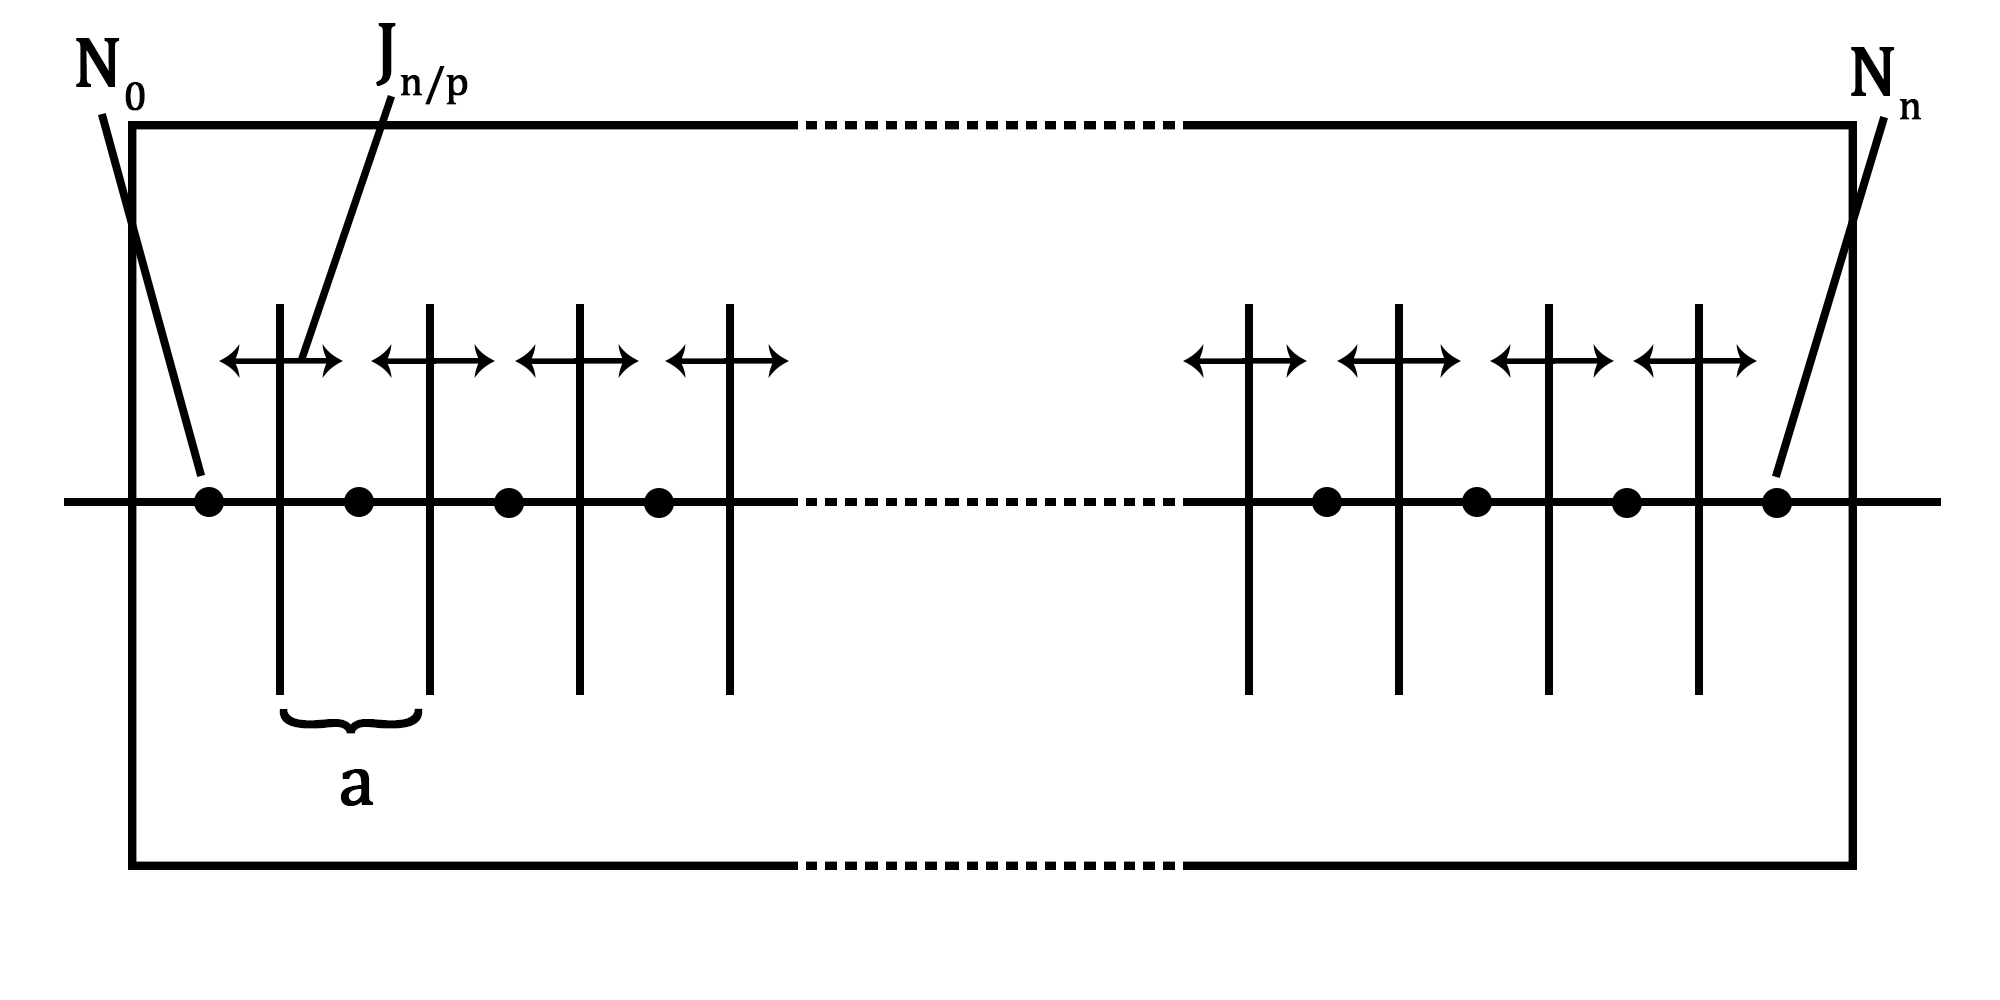
\includegraphics[scale=0.15]{Figures/Segmented}
	\caption{\label{fig:Mic:Segment}Visual representation of Microscopic model's segmented device. $N_x$ is node at position x, $a$ is the node width, and $J_{n/p}$ is the current density between two nodes for either electrons($n$), or holes($p$).}
	\hrule
\end{figure}
Each "node" along the device has a set width, $a$, and contain several variables and constants: The charge densities for electrons and holes ($n$ and $p$ respectively), and the potential at that point $V$ being the variables, and with constants determining doping of acceptor atoms $N_a$, doping of donor atoms $N_d$, and the Conduction and valence band relative energies, $E_c$ and $E_v$ respectively. \\
The device would be constructed as a "string" of these Nodes, with a set length, and area perpendicular to the current, which would limit it strictly to cuboid shaped devices. \\
Due the increased complexity of this model, there are more initial conditions to be considered, such as how many nodes there are, the specifications of each of the nodes, the overall dimensions and parameters of the device, etc. so the program running this simulation was designed to have similarly broad functionality. A command-line interface was built to allow a user to do the following tasks: load and save a "device" to file, bring a device to equillibrium, run the simulation on a device for a set of conditions, and run the a range of simulations for a range of conditions to calculate a range of photon pulses for different transition times to find the how the FWHM varied with number of photons in a pulse. \\
\subsubsection{Converting the equations to numerical form}
In order to do calculation using the Drift-Diffusion and Poisson's equations, they first had to be discretised. This could be achieved through the use of Taylor expansion's.\cite{Nkonga}\cite{ECE606}\\
Using the Taylor expansions of:
\begin{eqnarray}
	f(x+\delta x) &= f(x) + \delta x\dfrac{df}{dx}\Big|_{x = x+\delta x} + (\delta x)^2 \dfrac{d^2f}{dx^2}\Big|_{x = x+\delta x} + ...\\
	f(x-\delta x) &= f(x) - \delta x\dfrac{df}{dx}\Big|_{x = x-\delta x} + (\delta x)^2 \dfrac{d^2f}{dx^2}\Big|_{x = x-\delta x} - ...\\
\end{eqnarray}
it was possible to find approximations for both first a second derivatives by using:
\begin{eqnarray}
	\dfrac{df}{dx}\Big|_{x+\delta x/2} =& \frac{f(x+\delta x)-f(x-\delta x)}{\delta x}\\
	\dfrac{d^2f}{dx^2}\Big|_{x_i} =&  \dfrac{f(x+\delta x) + f(x-\delta x) - 2f(x_i)}{(\delta x)^2} 
\end{eqnarray}
Using these approximations, it was possible use Gauss' law to find the potential at each node point using:\cite{ECE606}
\begin{eqnarray}
	&\nabla\cdot\vec{D} = \rho \\
	&\nabla^2 \cdot V = \dfrac{\rho}{\epsilon_r \epsilon_0} \\
	&\nabla^2 \cdot V = \dfrac{V_{i+1}+V_{i-1}-2V_i}{a^2} \\
	\hookrightarrow & \dfrac{V_{i+1}+V_{i-1}-2V_i}{a^2} = \dfrac{\rho}{\epsilon_r \epsilon_0}\\
	& \dfrac{V_{i+1}+V_{i-1}-2V_i}{a^2} = \dfrac{q}{\epsilon_r \epsilon_0}(p+N_D-n-N_A)
\end{eqnarray}
Where $i$ indicates the node index. Using the same method, current densities $J_n$ and $J_p$ can be calculated thus:
\begin{eqnarray}
	J_n =& -q\mu_n(\dfrac{n_{i+1}+n_{i}}{2})(\dfrac{V_{i+1}-V_{i}}{a})\\
	 +& \mu_n (\dfrac{n_{i+1}+n_{i}}{2})(\dfrac{E_{c(i+1)}-E_{c(i)}}{a}) + qD_n(\dfrac{n_{i+1}-n_{i}}{a}) \\
	J_p =& -q\mu_p(\dfrac{p_{i+1}+p_{i}}{2})(\dfrac{V_{i+1}-V_{i}}{a})\\
	 +& \mu_p (\dfrac{p_{i+1}+p_{i}}{2})(\dfrac{E_{v(i+1)}-E_{v(i)}}{a}) - qD_p(\dfrac{p_{i+1}-p_{i}}{a}) \\
\end{eqnarray}
These three equations form the basis for the equilibrium and simulation abilities of the program.
\subsubsection{Program functionality: Saving \& Loading}
To allow use of user defined devices in the simulation process, a method of inputting the data rather than having it hard coded was necessary. To achieve this, a loading and saving method was designed.\\
A specific \textit{.csv} file format was developed that could be read by the program. An overview of the specifics of the format can be found in the \textbf{APPENDIX: TODO} to allow for the reader to create their own. This file would contain all the necessary information to create a device in the program, including: device length, area, resistance, number of nodes, and each of the individual node's data. To enable ease of reading for the program, a second internal file-type was created based on this file called a "doesn't include commas" file that was, in essence, this specifically structured .csv file type with all commas removed. This .dic file was easier to read and less error prone on reading, and would be automatically generated by the program.\\
The program could also save the current device in memory to a .csv file in the correct format to be transported, permanently recorded, or opened in an external spreadsheet or text editor program. This makes editing or altering device data far easier for the user.
\subsubsection{Program functionality: Equillibrium}
Once a device has been loaded into the program, the user is able to bring the device to "equilibrium". This is done by running the continuity equation simulation on the device with no external input until a minimum total internal current is reached (defined by the user, recommended $\approx 1cm^{-3}s^{-1}$ or less) where total internal current is defined by:
\begin{eqnarray}
	&J_{tot} = \sum\limits_{i=1}^{n}J_i\\
	&J_i = J_{n(i)}+J_{p(i)}
\end{eqnarray}
 This step is important to ensure the calculations have the intended behaviour and that running a simulation cycle doesn't result in excess photons being released from the device not already being in steady-state equilibrium. The following algorithm was used to achieve this:
\begin{algorithm}
	\While{$J_{tot} < tolerance$}
	{
		Calculate V at each node\;
		Calculate $J_n$ between each node and transfer charge density\;
		Calculate $J_p$ between each node and transfer charge density\;
		Cancel any charges that would recombine\;
		$J_{tot} = \sum J_{n(i)}+J_{p(i)}$
	}
\caption{\label{alg:mic:Eqm}Algorithm for bringed device to equillibrium}
\end{algorithm}
As running this algorithm at standard $J$ values would be very slow, a user-defined "Approximation" multiplier is used to speed this process up (typically a value from $10^3$ to $10^6$ is recommended.) This multiplier simply takes what the exchange current $J$ would be, and multiplies it by this value. Very large values has undefined behaviour, and in such cases, reloading the device from file is necessary, but without it, this process could take many millions of iterations. \\
Though not used in the final program, the code has debug functionality to print device status to file and console whilst this is happening, as well as print $J_tot$ to file for each iteration.

\subsubsection{Program functionality: Single simulation}
Using many of the same principles as the "Macroscopic" device model program and its algorithms, this command takes the device loaded and injects charges following the voltage tent map, and Ohmic D.C. modelling. It uses exactly the same code for finding FWHM of the pulse, though due to fundamental differences in design, the algorithms for finding the number of photons released from recombination are slightly different.\\
From device equilibrium where:
\begin{eqnarray}
	&n_R(t=0) = 0\\
	&J_{tot}(t=0) \approx 0\\
	\hookrightarrow &\dfrac{dn}{dt}\Big|_{t=0} \approx 0
\end{eqnarray}
and same for holes, injection of electrons from one end and holes from the other can begin.\\
This is done in the same time-step like manner of the Macroscopic device, however the algorithm is adjusted to:\\
\begin{algorithm}[H]
	\While{$n_R \geq 0$}
	{
		Add $t_step$ to $t$\;
		Find V at $t$\;
		Find $J_{input}$ from V\;
		Find $V_i$ for each node\;
		Propagate $n$ and $p$ through device with $J_n$ and $J_p$\;
		Find $n_R$ at each node and remove respective charge densities\;
		Save $n_R$ to histogram bin arrays\;
		Save respective $t$ to corresponding array\;
	}
	Find FWHM using Algorithm \ref{alg:Mac:FWHM}\;
	\caption{\label{alg:Mic:Inner} Segmented device single simulation run algorithm.}
\end{algorithm}
In the case where the external bias Voltage is reversed, so will be the $J_{input}$ current density, pulling that charges from that end of the device where 
\begin{equation}
	J_{input} = \frac{V}{AR}
\end{equation}
where $A$ is the area perpendicular to the direction of current.\\
\subsubsection{Program functionality: Full simulation}
This command treats the single simulation as the Macro model would treat the "inner loop" algorithm (see Algorithm \ref{alg:Mac:inner}) and in this respect, the Full simulation command is much like the "outer loop" algorithm (see Algorithm \ref{alg:Mac:outer}).\\
The same basis of incrementing the transition time in a stepwise fashion to find the associated FWHM and number of photons until reaching a maximum transition time is employed. However, due to the device being left in a state of none-equilibrium between each run, it has to be reloaded from file between each iteration. The algorithm is as follows:\\
\begin{algorithm}[H]
	\For{$t_{trans} =0$ to $t_{trans}=t_{transMax}$}
	{
		Load device in equilibrium\;
		Single iteration simulation (Algorithm \ref{alg:Mic:Inner})\;
		Log both FWHM and $n_R$\;
	}
	Save FWHM and $n_R$ arrays to file\;
	\caption{\label{alg:Mic:Outer} Segmented device full ranged simulation algorithm.}
\end{algorithm}
in which the transition time maximum, step, and simulation time-step are defined by the user on command call.
\section{Results}
This section will simply contain any graphs of importance for model and real results, such as the $\sigma_{FWHM}(\ln(N_{\gamma}))$, $J_n(t)$, $J_n(x)$, potentially $N_{\gamma}(T)$ and the graph of n-doped and p-doped segments coming together and their $n(x,t)$ graph. \\ These will come with brief descriptions and overview of the data they contain including initial condition parameters, choices of constants, and references to the code in the appendix that generated them.
\section{Discussion}
In this section, the results of the modelling compared to real-world results will be discussed. Topics of interest will be: Does the model predict the $N_{\gamma} \propto t^{3} $ results instead of the linear response predicted by Windisch's instantaneous current model ( $N_{\gamma} \propto t^{2} $) or does it manage the closer to experimental result of $t^{4}$?\\
Discuss the model's simulated capacitance and whether it's similar to that measured experimentally, or predicted by \textbf{Veledar}.\\
Did the model produce any temperature dependency graphs for photon emission, and if so, how do they again compare to experimental results?

\section{Conclusion}
In this section talk about the limits of the model (only 1D, inaccuracies with reality, etc) and discuss known ways to improve it. Discuss reasons for them not already being implemented (lack of knowledge about device[read: band structure, dimension, composition], more accurate models much more time consuming to build, etc...) \\


\section{References}
This section will be filled automatically by using BibTeX once I've started putting together the .bib file.\\
I intend to reference in a similar form to standard reference, but include page number for each. For example:\\
\fbox{\begin{minipage}{10cm}
	...leads to the well known drift diffusion current[4](p305) [6](p108):
	\begin{equation}
	J_{n} = q \mu_n n \vec{E} + q D_n \Delta n
	\end{equation}
\end{minipage}}
\medbreak
Format requested: "Last name, First initial. (Year published). Article title. Journal, Volume (Issue)" \textbf{How do I get it in that form $\downarrow$ ?} \textbf{Im aware a couple of these haven't worked properly from Bibtex, I'll find a fix later.}
\bibliography{thesis_ref}{}
\bibliographystyle{ieeetr}
\bigskip

\section{Appendix}
\subsection{Code Overview: Micro}
\subsubsection{Current density calculation methods}
\begin{figure}
	\centering
	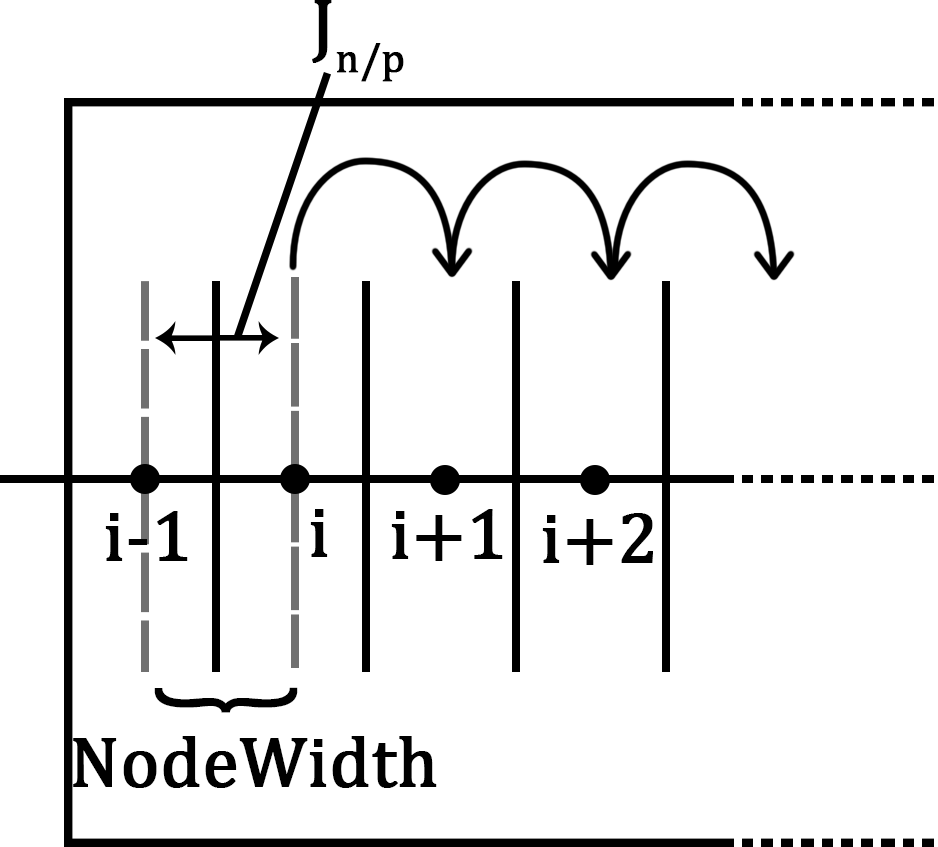
\includegraphics[scale=0.2]{Figures/JnL}
	\caption{\label{fig:Mic:JnL} Diagram of calculateJnLEC method's functionality.}
\end{figure}
This section contains the information on how current was calculated within the device.\\ Four functions were written, all with very similar structures but with alterations dependent on whether the order was starting from the left, or from the right, and whether it was done for the holes or electrons: JnL, JnR, JpL, and JpR. \\
For this example, JnL will be used to demonstrate the structure, with its depiction shown in Figure \ref{fig:Mic:JnL}.
The code worked by taking the device's std::vector<Node>s and manipulating the electron (or hole) densities by applying:
\begin{eqnarray}
	&J_n = -q\mu_n n\nabla V + \mu_n n \nabla E_c + q D_n \nabla n\\
		\hookrightarrow &J_n = -q\mu_n(\dfrac{n_{i+1}+n_{i}}{2})(\dfrac{V_{i+1}-V_{i}}{a})\\
	+& \mu_n (\dfrac{n_{i+1}+n_{i}}{2})(\dfrac{E_{c(i+1)}-E_{c(i)}}{a}) + qD_n(\dfrac{n_{i+1}-n_{i}}{a}) \\
\end{eqnarray}
starting from the second node, to the last in that order, calculating the current between the node, and the that of the one to its left.\\
Line 3 creates a variable to store the absolute value of the current between the two nodes and adds it to a cumulative value to be returned once the function is complete. This return is used in parts of the program to guage whether the device is in equilibrium or not.\\
Lines 11 and 12 simply find the current and transfer the difference from one to other with correct dependence depending on the direction of the current density.\\
The exchange scale multiplies this transfer which results in significantly fewer loops required where time is not a factor in the calculation. As current density is charge transfer per unit time, it also works as a crude method of integrating the current calculation over a time period, treating it as constant current.\\
By using this approximation method, it is only valid for relatively small approximations where $J_{nL} t \ll n$ and is the equivalent of doing:
\begin{equation}
 \sum\limits_{i=1}^{x}\dfrac{dn}{dt}\Big|_{t=t_i} = \lim\limits_{n''(t)\to 0} x* \dfrac{dn}{dt}\Big|_{t=t_1}  
\end{equation}
and is assumed that the rate in change in current transfer is smooth and small as to allow for this approximation. Because, in this approximation, $\frac{dn}{dt}$ is only needed to be calculated once, this is far faster for use in the equilibrium code by applying an approximation factor.
\begin{lstlisting}[caption = Example of the current calculation algorithm]
double Device_1D::calculateJnLEC(double exchangeScale)
{
	double JnL_cum = 0;	
	for (std::size_t i = 1; i < nAry.size(); i++)
	{
		double dn = (nAry[i].n - nAry[i - 1].n) / nodeWidth;
		double dV = (nAry[i].V - nAry[i - 1].V) / nodeWidth;
		double dEc = (nAry[i].Ec - nAry[i - 1].Ev) / nodeWidth;
		double n = (nAry[i].n + nAry[i - 1].n) / 2;
		double JnL = (-q * mu*n*dV) - (mu*n*dEc) + (q*D*dn);
		nAry[i].n = nAry[i].n - (JnL*exchangeScale);
		nAry[i - 1].n = nAry[i - 1].n + (JnL*exchangeScale);
		JnL_cum += abs(JnL);
	}
	return JnL_cum;
}
\end{lstlisting}



In this section I will include any data I may have, and include all\textbf{(?)} the code produced for the project. An example code snippet to demonstrate formatting:\smallskip
\begin{lstlisting}[caption = Hello world example code.]
	int main()
	{
		std::cout<<"Hello world!"<<std::endl;
	}
\end{lstlisting}
\medskip
An example of some raw data would be formatted into a table as such:\\
\begin{table}[h]
	\centering
	\begin{tabular}{|l|c|c|}
		\hline
		\textbf{Name} & \textbf{A} & \textbf{B} \\
		\hline
		First & 1 & 2 \\
		Second & 3 & 4 \\
		\hline
	\end{tabular}
	\caption{\label{tab:appendixTest} This table is purely for demonstration of format.}
\end{table}
and will be referenced in the text as such[Table:\ref{tab:appendixTest}].
\end{document}
